
\section{Introduction}

\begin{frame}{}
    \begin{figure}[htpb]
        \centering
        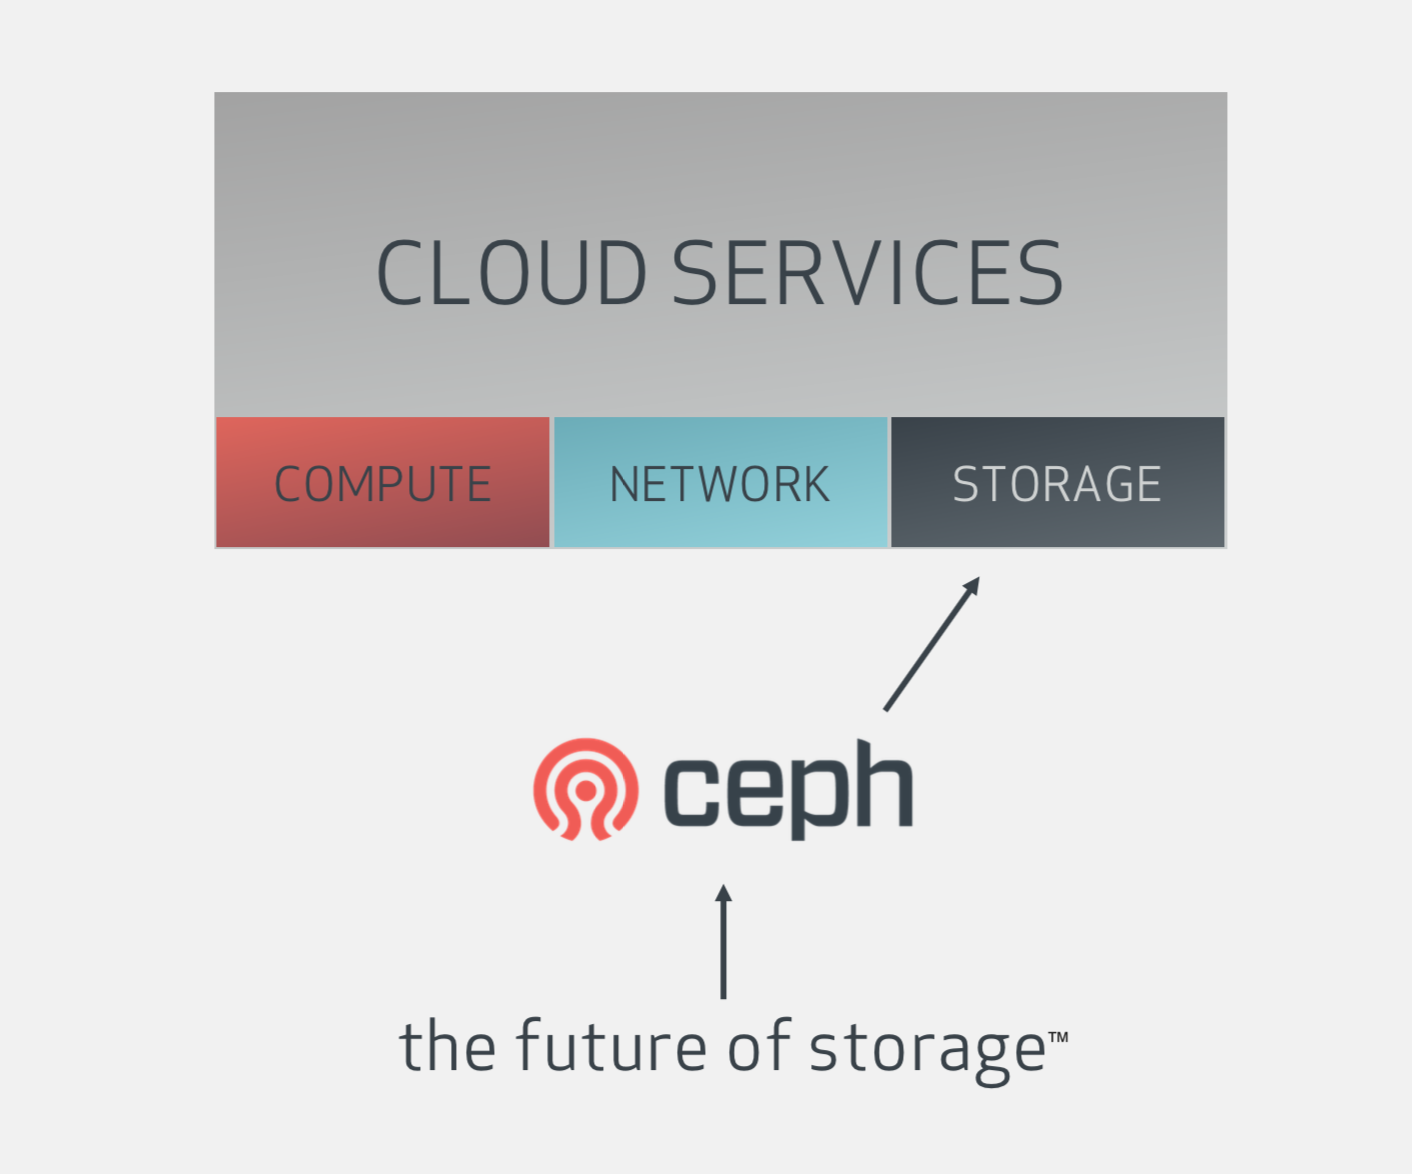
\includegraphics[width=0.7\linewidth]{future-of-storage.png}
    \end{figure}
\end{frame}

\begin{frame}{Timeline of Ceph}
    Original author: \textbf{sage weil}
    \begin{figure}[htpb]
        \centering
        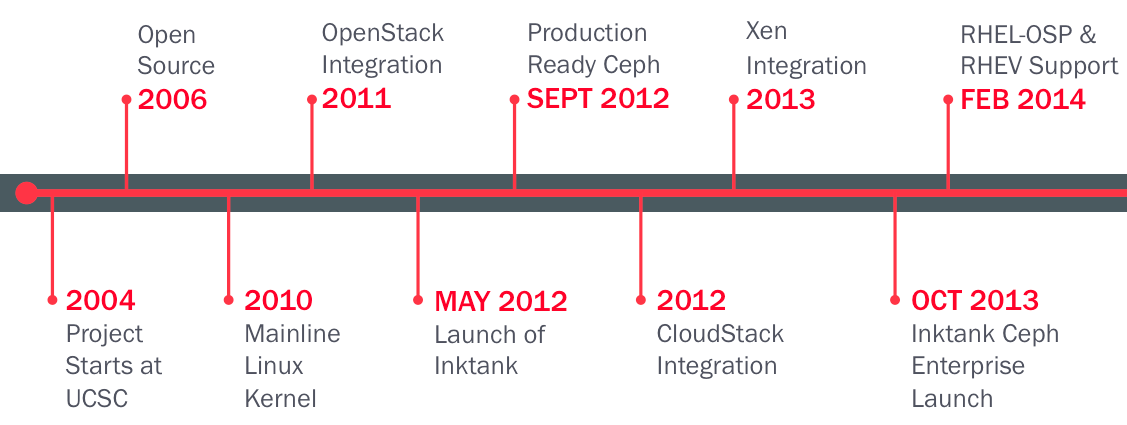
\includegraphics[width=0.8\linewidth]{timeline.png}
    \end{figure}
\end{frame}

\begin{frame}{}
    \begin{figure}[htpb]
        \centering
        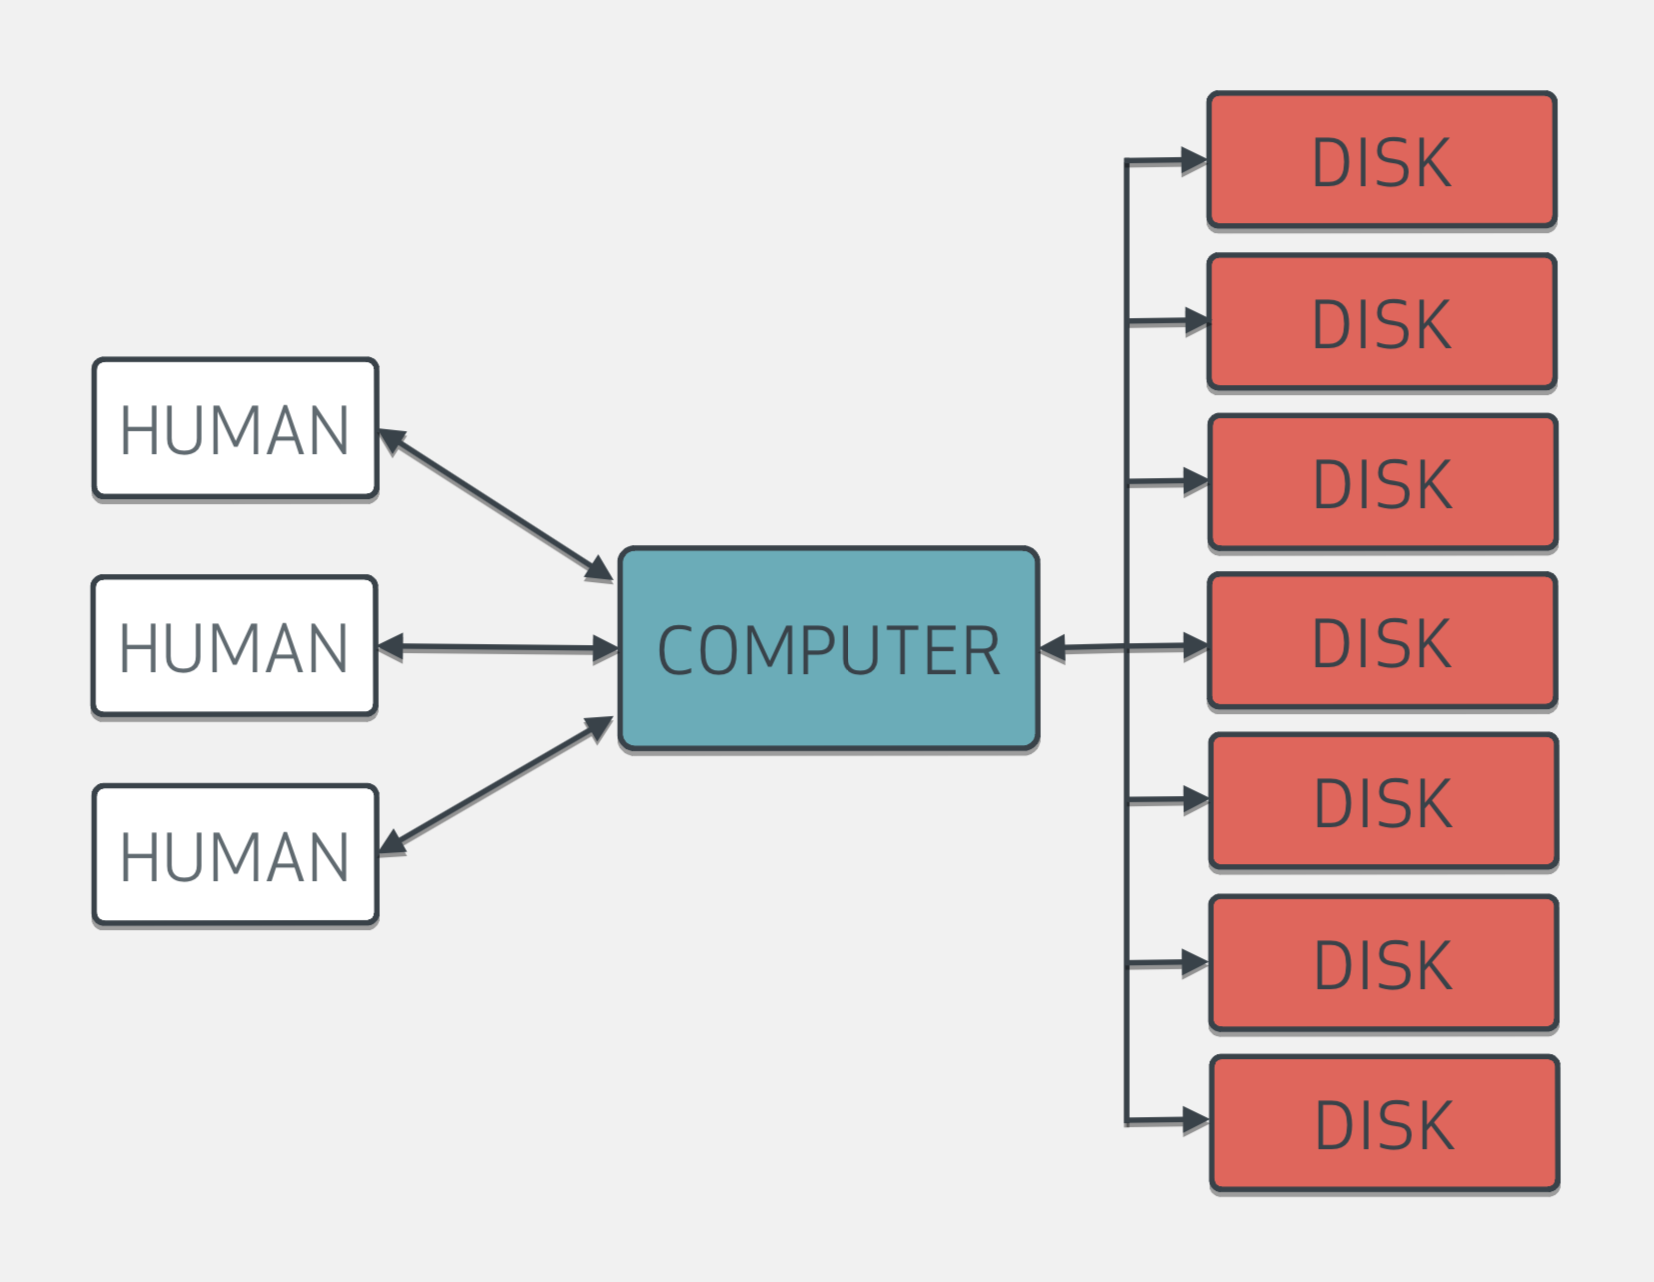
\includegraphics[width=0.7\linewidth]{storage1.png}
    \end{figure}
\end{frame}

\begin{frame}{}
    \begin{figure}[htpb]
        \centering
        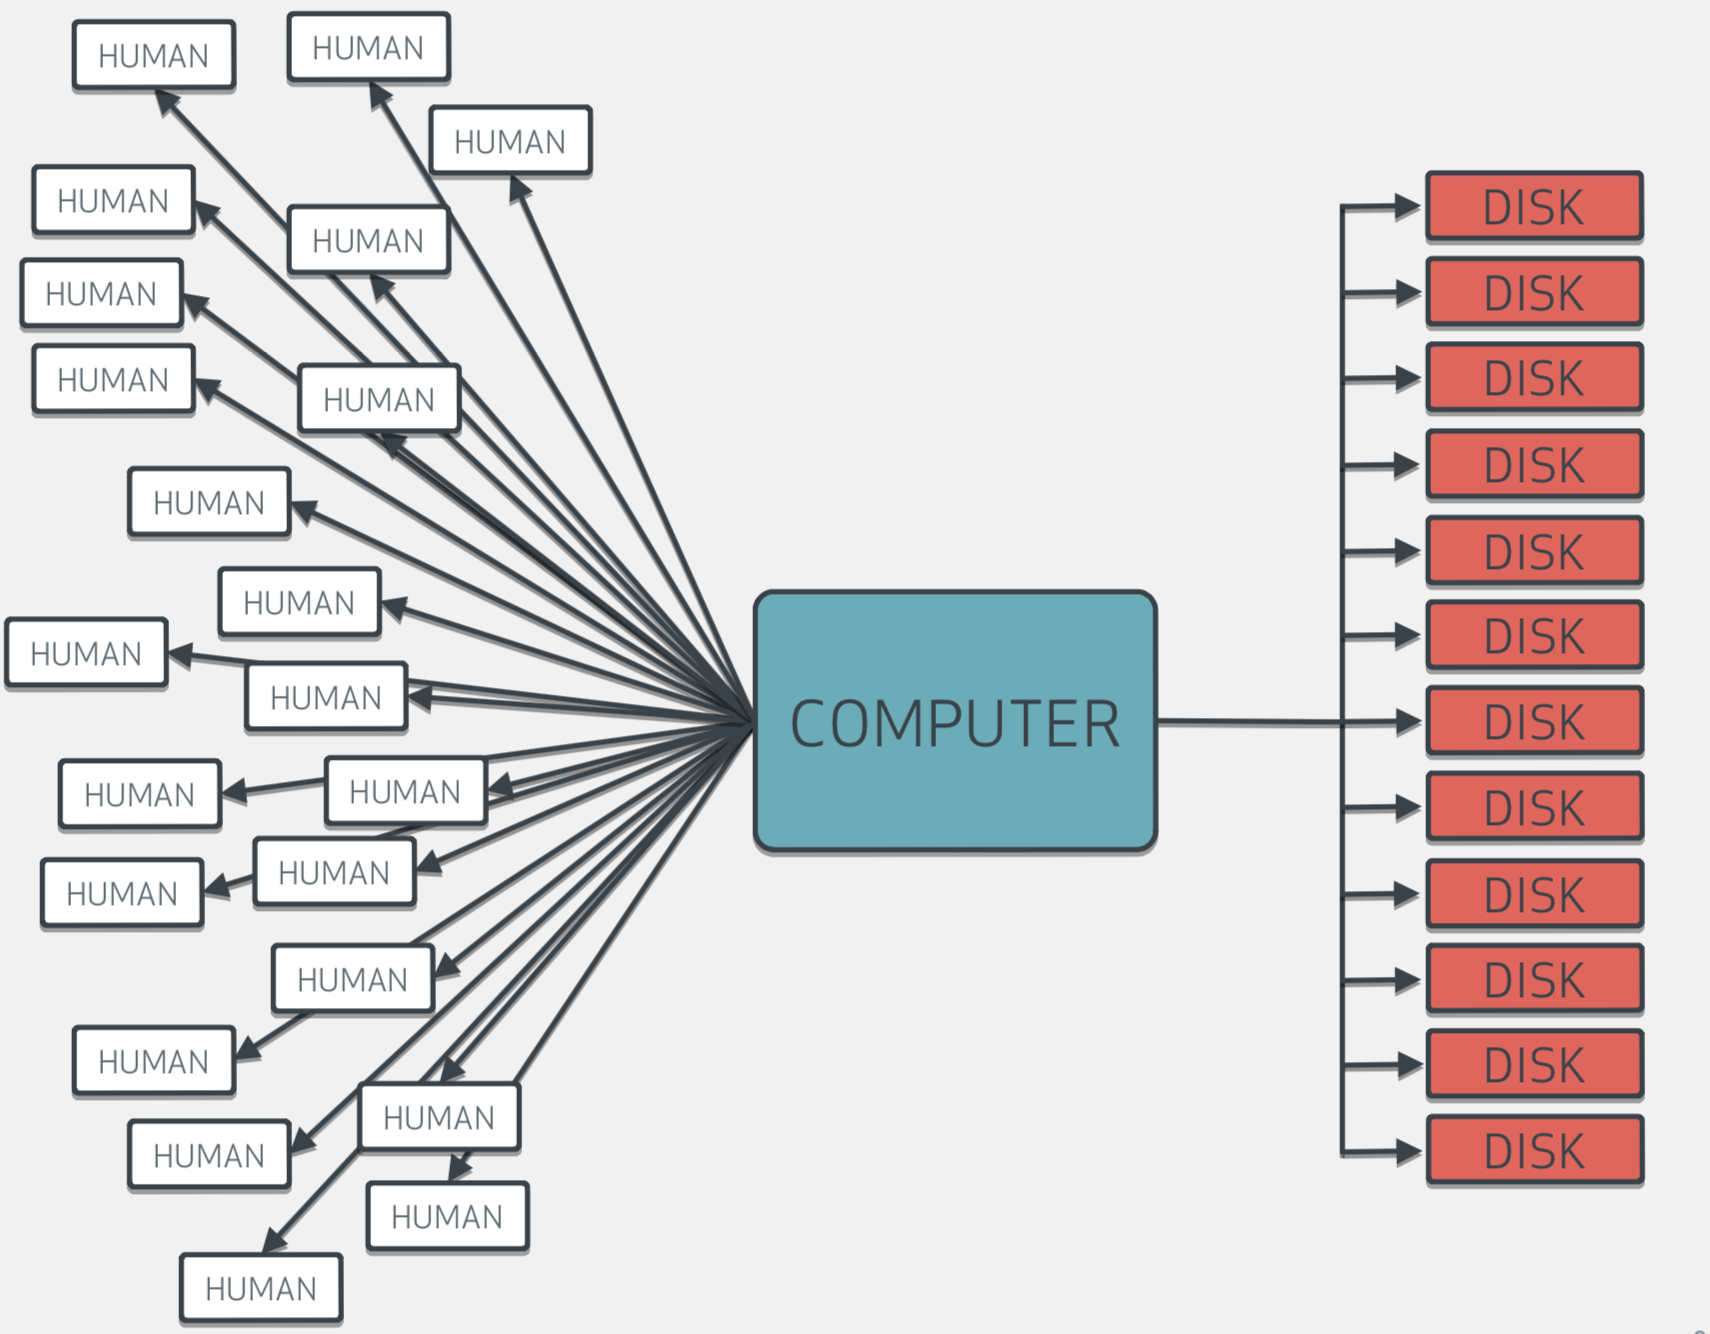
\includegraphics[width=0.7\linewidth]{storage2.png}
    \end{figure}
\end{frame}

\begin{frame}{}
    \begin{figure}[htpb]
        \centering
        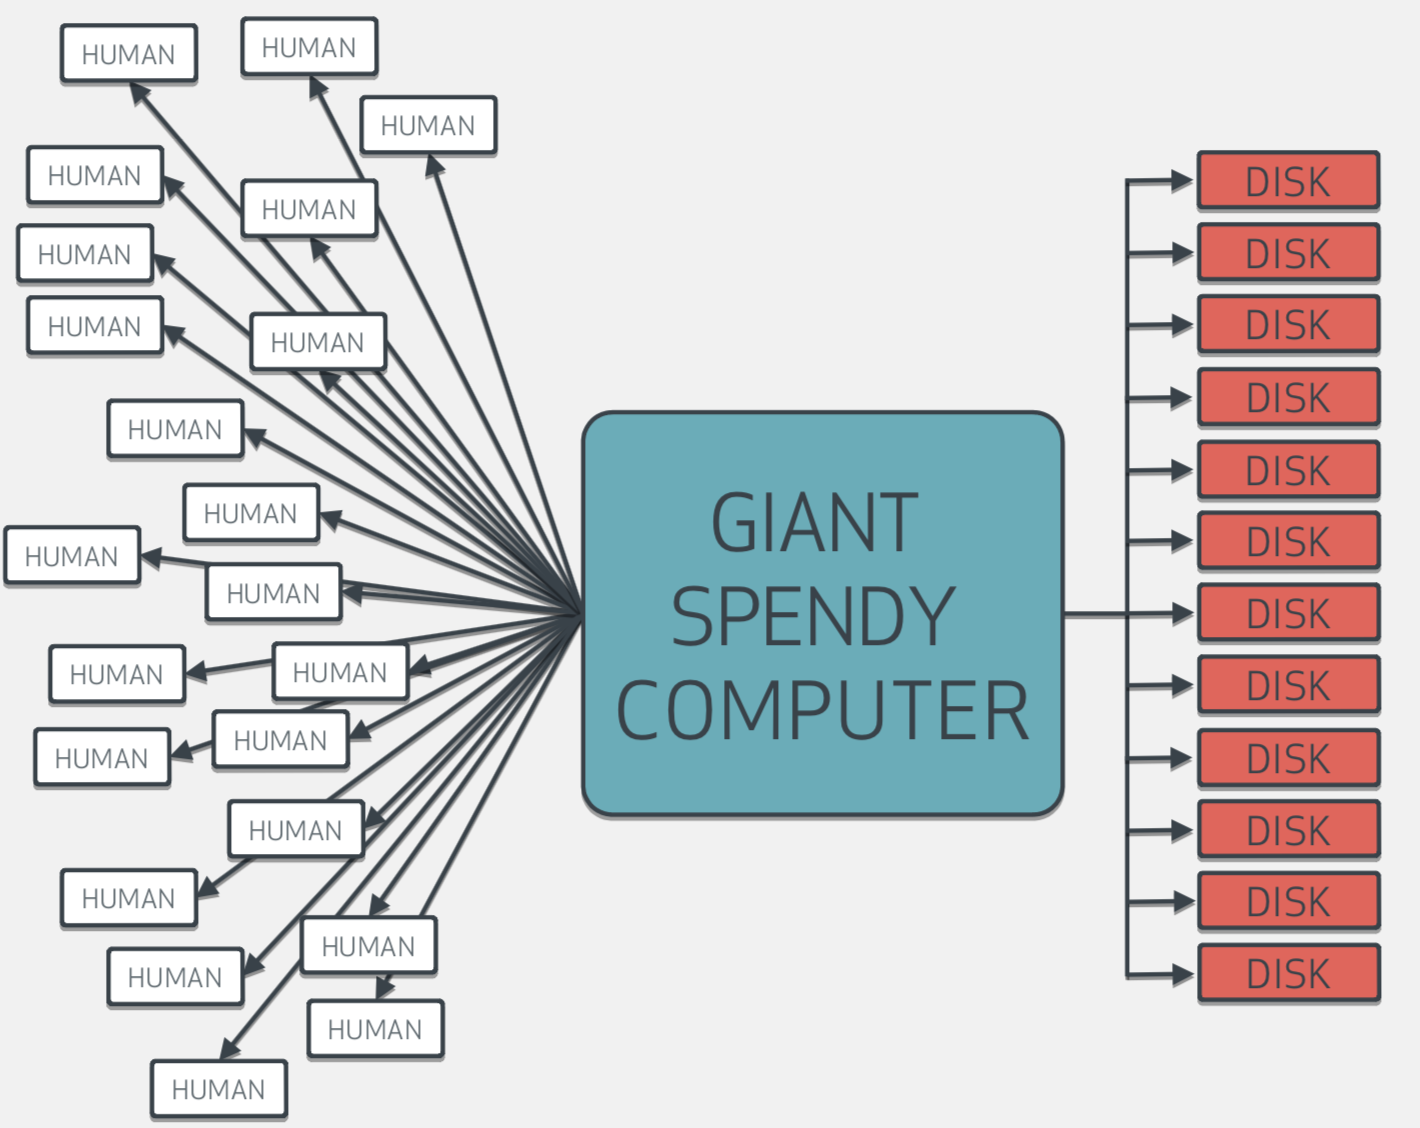
\includegraphics[width=0.7\linewidth]{storage3.png}
    \end{figure}
\end{frame}

\begin{frame}{}
    \begin{figure}[htpb]
        \centering
        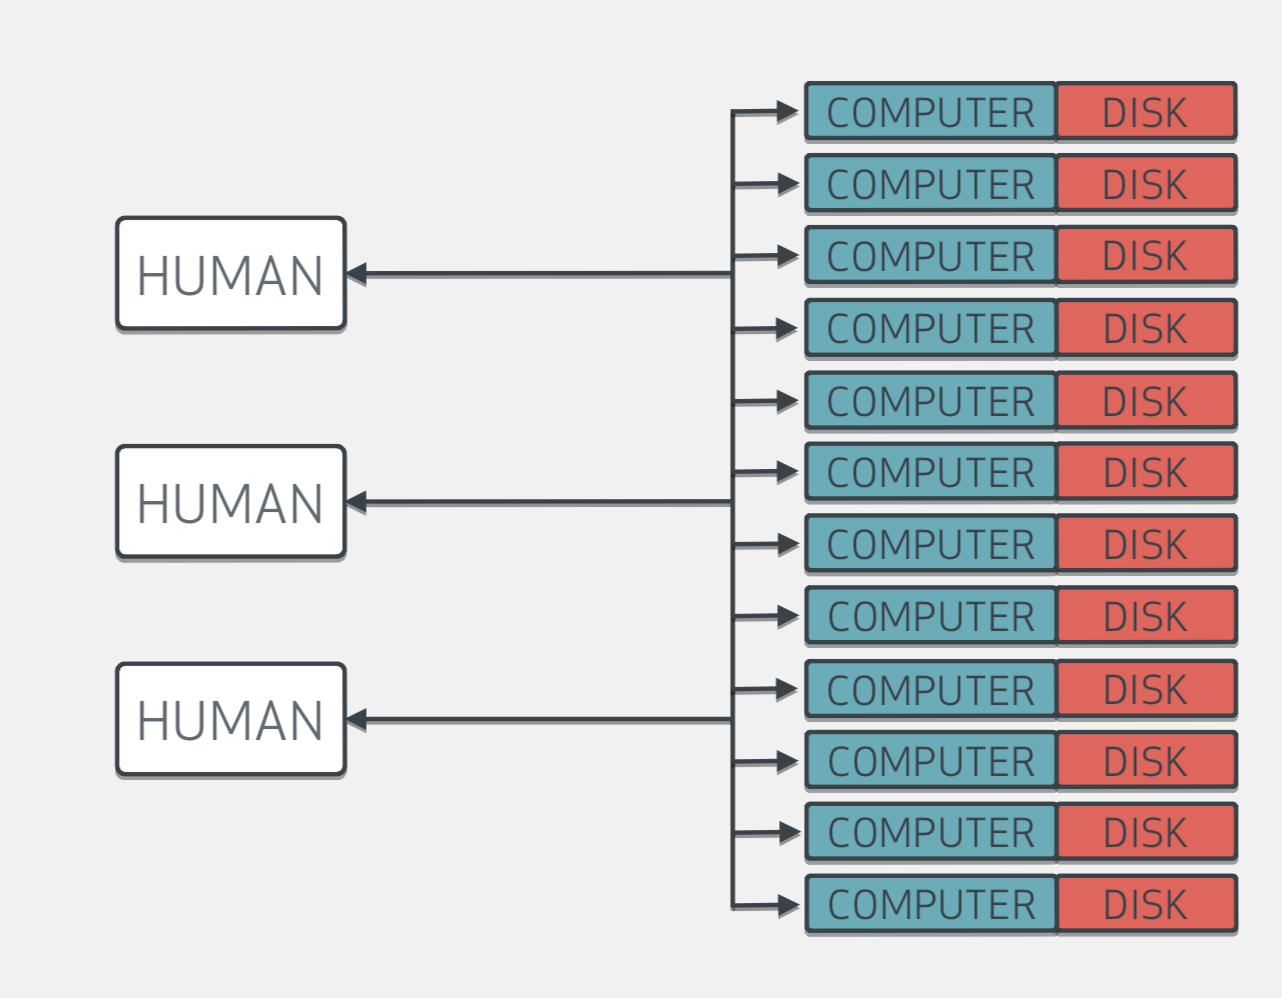
\includegraphics[width=0.7\linewidth]{storage4.png}
    \end{figure}
\end{frame}

\begin{frame}{}
    \begin{figure}[htpb]
        \centering
        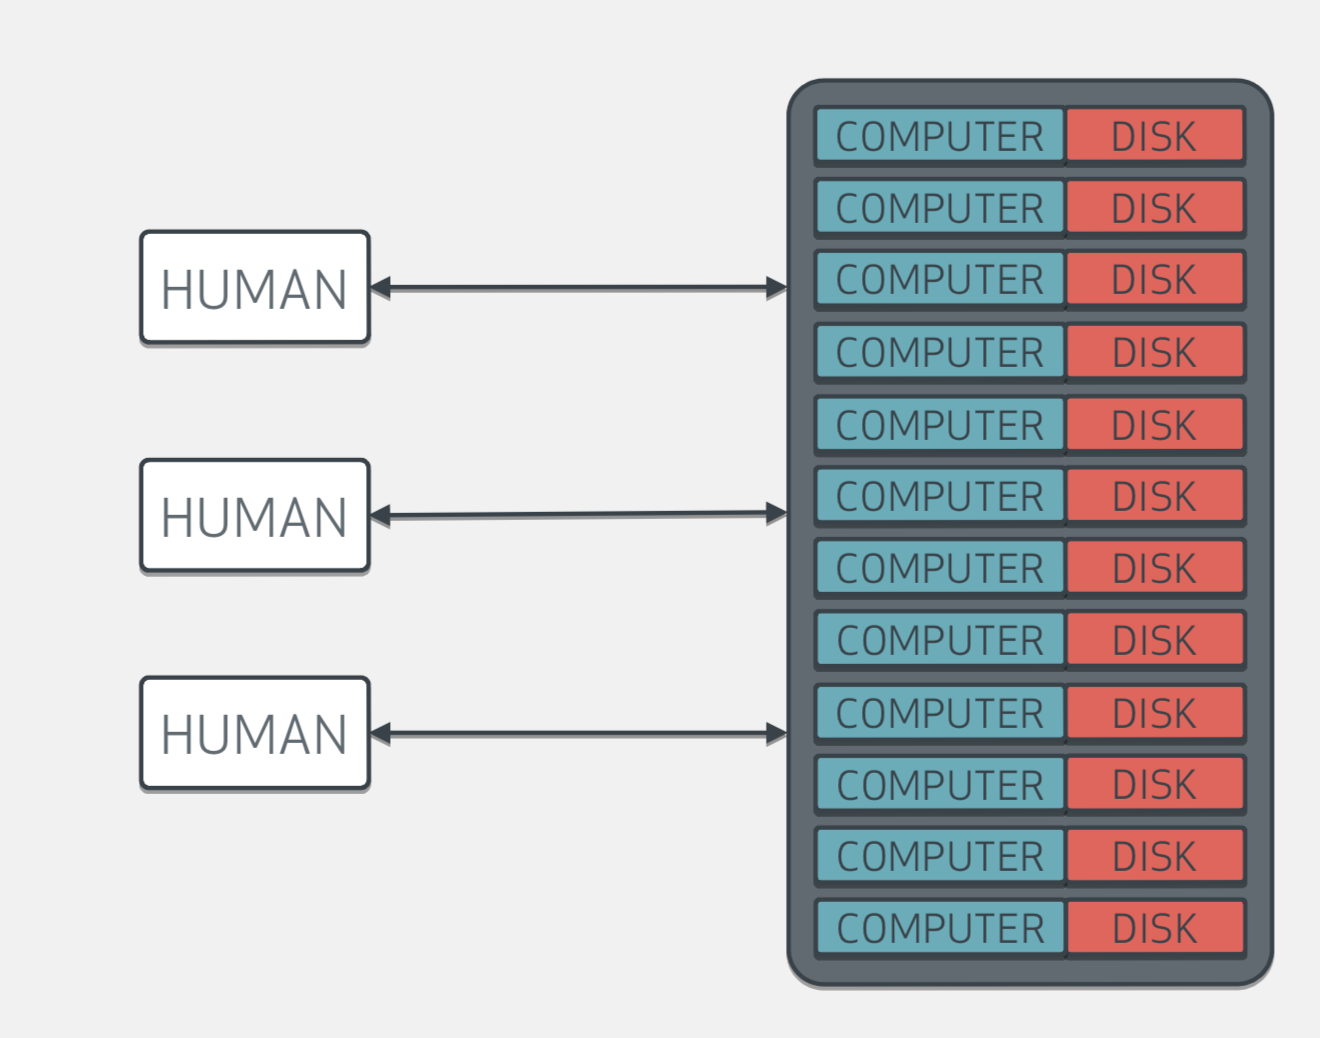
\includegraphics[width=0.7\linewidth]{storage5.png}
    \end{figure}
\end{frame}

\begin{frame}{}
    \begin{figure}[htpb]
        \centering
        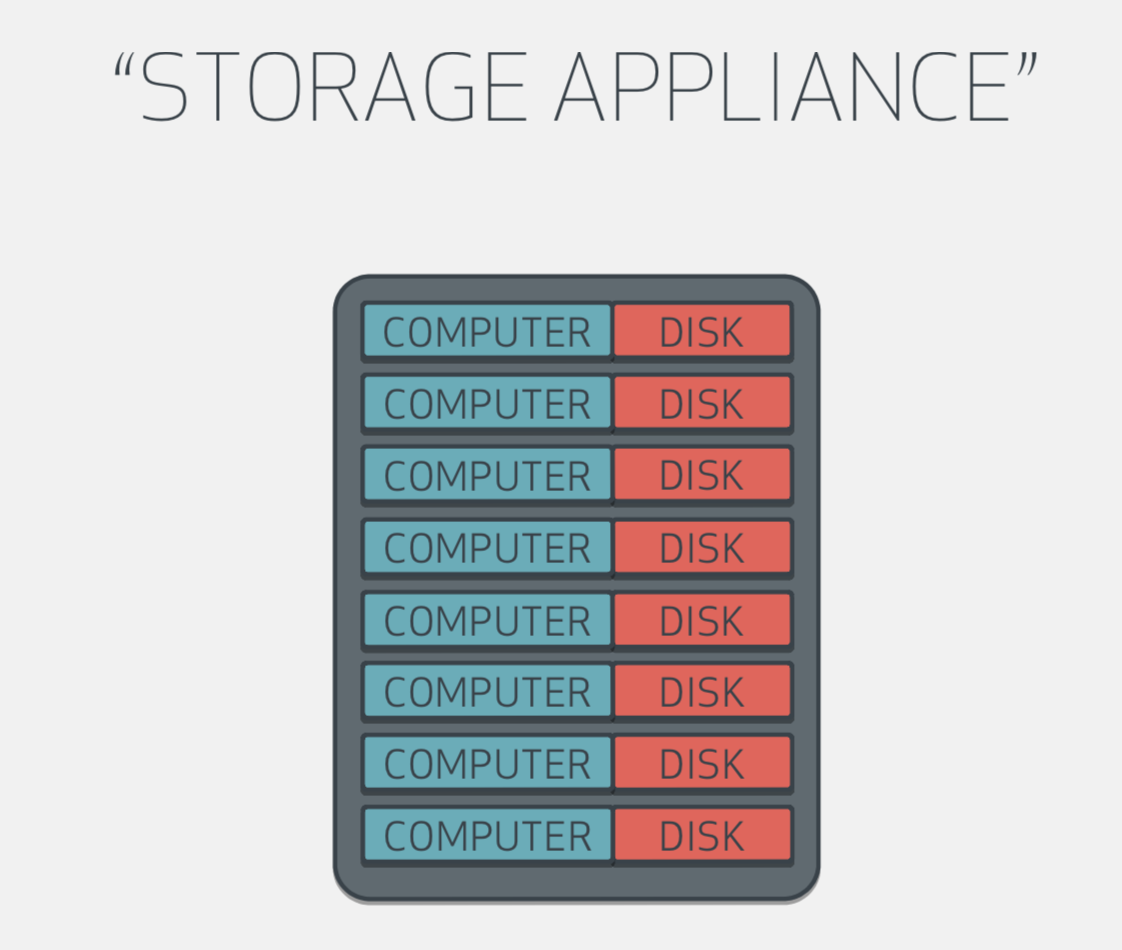
\includegraphics[width=0.7\linewidth]{storage6.png}
    \end{figure}
\end{frame}

\begin{frame}{Storage Challenges}
    \begin{itemize}
        \item \textbf{Must Support Current Infrastructures}
            \begin{itemize}
                \item Block storage with snapshots, cloning
                \item File storage with POSIX support
            \end{itemize}
        \item \textbf{Must plan for integration of emerging technologies}
            \begin{itemize}
                \item Cloud infrastructures and SDNs
            \end{itemize}
        \item \textbf{Must Support New Challenges}
            \begin{itemize}
                \item Object storage to support massive influx of unstructured data
            \end{itemize}
        \item All this while supporting:
            \begin{itemize}
                \item \textbf{Massive data growth -> scalability}
                \item \textbf{Mixed hardware that must work heterogeneously}
                \item \textbf{Maintain reliability and fault tolerance}
                \item \textbf{Performance!} 
            \end{itemize}
    \end{itemize}
\end{frame}

\begin{frame}[t]{Ceph Features}
    \begin{itemize}
        \item \textbf{Hardware Agnostic} \\
            Runs on commodity servers with directly attached storage. Not locked in a specified hardware platform.
        \item \textbf{Flexible} \\
            Can define pools of storage with differenct redundancy rules, disk types, geographic placement, depending on user requirements.
        \item \textbf{Scalable} \\
            In both bandwidth and capacity. No metadata servers. Silent clients do not generate network traffic/cluster load.
        \item \textbf{Self-Healing} \\
            Recovers automatically after disk or server failures.
    \end{itemize}
\end{frame}

\begin{frame}
    \frametitle{Ceph: Unified File Storage}
    \begin{itemize}
        \item \textbf{Object}
            \begin{itemize}
                \item Native LIBRADOS (Reliable Autonomic Distributed Object Store)
                \item RADOS Gateway provides S3/Swift REST API compatibility
            \end{itemize}
        \item \textbf{Block}
            \begin{itemize}
                \item Linux kernel (krbd) and KVM(librbd) support
                \item provides snapshotting and cloning capabilities
            \end{itemize}
        \item \textbf{File}
            \begin{itemize}
                \item CephFS support file system
            \end{itemize}
    \end{itemize}
\end{frame}

\begin{frame}[t]{Ceph Stack}
    \begin{figure}[htpb]
        \centering
        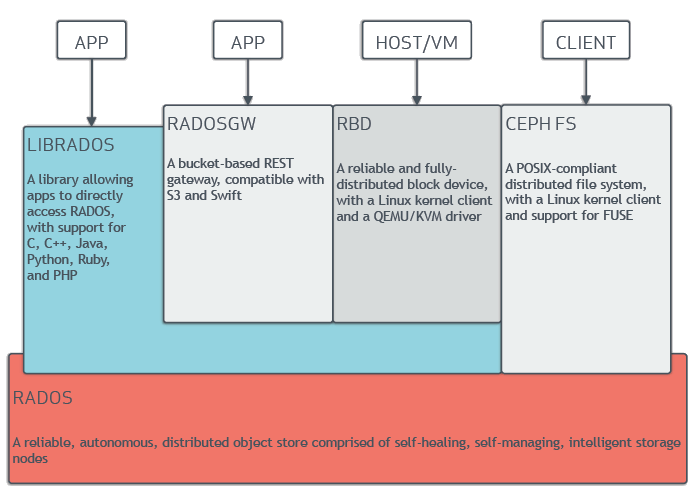
\includegraphics[width=0.75\linewidth]{stack.png}
        \caption{Ceph Stack}
        \label{fig:stack}
    \end{figure}
\end{frame}

%\begin{frame}[t]{Ceph Storage Cluster}
%    \textbf{A Ceph Cluster consist of:}
%    \begin{columns}
%        \begin{column}{0.4\textwidth}
%            \begin{itemize}
%                \item \textbf{Ceph Nodes}
%                    \begin{itemize}
%                        \item Each node hosts multiple OSDs
%                        \item Each OSD has:
%                            \begin{itemize}
%                                \item 1 hard disk
%                                \item 1 xfs file system
%                                \item 1 Ceph OSD daemon
%                                \item (optional) journal hosted on a separated SSD
%                            \end{itemize}
%                    \end{itemize}
%                \item \textbf{Monitors}
%                \item \textbf{Optional RADOSGW for providing S3/Swift compatibility} 
%            \end{itemize}
%        \end{column}
%        \begin{column}{0.6\textwidth}
%            \begin{figure}[htbp]
%                \centering
%                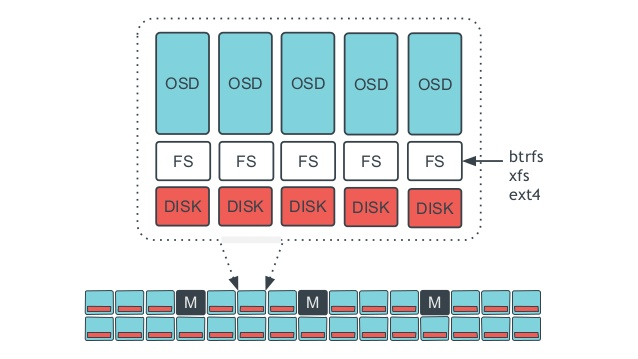
\includegraphics[width=1\linewidth]{cluster.jpg}
%            \end{figure}
%        \end{column}
%    \end{columns}
%\end{frame}
%
